\chapter{Indexing for Incremental Proof Development}

\newcommand{\private}[1]{#1_\downarrow}
\newcommand{\public}[1]{#1_\uparrow}
\newcommand{\Private}[1]{#1_\Downarrow}
\newcommand{\Public}[1]{#1_\Uparrow}
\newcommand{\Env}{\Xi}
\newcommand{\Frame}{\mathbb{F}}
\newcommand{\Module}{\mathbb{M}}
\newcommand{\Pattern}{\mathbb{P}}
\newcommand{\Entry}{\mathbb{E}}
\newcommand{\Var}{\mathbb{V}}
\newcommand{\Constant}{\mathbb{C}}
\newcommand{\Fail}{\lightning}
\newcommand{\Lookup}[2]{\operatorname{lookup}\left[#1\right]\left(#2\right)}
\newcommand{\Index}{\operatorname{index}}
\newcommand{\Domain}{\operatorname{domain}}
\newcommand{\Pop}[2]{\operatorname{pop}\left[#1\right]\left(#2\right)}
\newcommand{\Translates}{\rightsquigarrow}

This chapter presents implementation concerns with supporting incremental program development in \Beluga and \Harpoon.
Some technical debt in those systems is highlighted to justify the reimplementation of the indexing phase.
A formalism and an implementation of identifier resolution in \Beluga are presented to showcase how to efficiently and correctly support de Bruijn indices with multiple indexing contexts.

\section{Introduction}

% What are aspects of state management that are required to support incremental proof development?
% In what way are state management and exception handling closely linked with respect to interactive proof sessions?

% TODO: Talk about trailing, snapshot mechanisms, soundness preservation, ...
Incremental program development is a broad and open problem in the implementation of interpreters and compilers.

Structured editing obviates some of the issues with cache invalidation and the propagation of changes in incremental development.
Indeed, edit actions are scoped to a model of the program as opposed to the program's textual representation itself, which means they have a limited and controlled effect on the structured editor's state.

% TODO:

% How do other systems supporting interactive proof sessions handle state management?

Proof assistants providing interactivity through \acp{REPL} or tools for text editors each approach the problem of incremental development in unique ways tailored to their systems.
For instance, constraint-based type systems require trailing mechanisms to revert state changes induced by solving type constraints on new and pre-existing type variables when type-checking fails for a given program.
Likewise, context-switching between different parts of a program under edit requires updating the state to correctly reflect what identifiers are in scope.
Furthermore, in proof assistants specifically, command histories may be implemented to support undoing and redoing commands or tactics.
Subgoal trees may also added to allow navigating between incomplete parts of a proof.
The successful implementation of these structured editing features hinges on careful management of recorded state.

The \Abella\footnote{\Abella version \texttt{2.0.8}}~\cite{baelde2014abella} interactive theorem prover has limited support for structurally editing proofs.
Indeed, it leverages a single global state comprised of mutable references with a snapshot mechanism to copy the entire state on every undoable command.
This state notably includes the signature of declarations, the subordination relation on type families, and the list of subgoals that have yet to be proven in the current lemma under edit.
Hence in its interactive mode, \Abella users are restricted to adding new declarations at the end of the session's state.
Indeed, constructing visiting states to other parts of the signature under edit would require rerunning the processing pipeline.

\Isabelle/\Isar\footnote{\Isabelle2023} implements a system of transitions between immutable state structures to support pure edit actions~\cite{wenzel2023isabelleimpl, wenzel2023isabelleisarref, wenzel2023isabellesys}.
Indeed, most of that system's state, also called contexts~\cite{ballarin2006interpretation}, is implemented using immutable 2-3~trees to tabulate data, and each context holds a list of all predecessor states.
The definitions, proofs and terms in the buffer under edit are stored in such contexts.
Undo operations and modification to the signature then proceed by rolling back the contexts to before the edit was done using the list of predecessors.
Mutable references are leveraged to represent the global state of the kernel, though their usage is limited.
This mutable data is split between synchronized and unsynchronized management strategies, the former adding mutual exclusion locks to references that hold mutable data.
Overall, the extensive use of immutable data structures coupled with synchronization for mutable data result in degraded memory usage and runtime performance.
Nonetheless, this system allows finer edit actions and ensures that cache invalidations are resolved consistently.

\Agda\footnote{\Agda \texttt{v2.6.4}}~\cite{clffolp, norell2007towards, agda2023} supports incremental interactions through commands evaluated in its type checking monad.
Issuing a command in this \Agda mode directly affects the text editor's buffer, which provides a seamless editing experience.
In essence, the type checking monad is an instance of the state monad, whose state structure contains most of the mutable and immutable data used throughout the system.
This includes global configuration parameters, scope information, user-defined notations for parsing, typing contexts for variables as association lists, etc.
It is an agglomeration of all the data used in \Agda's processing pipeline, readily available as a function parameter as opposed to being represented using a global mutable data structure.
This wholly captures the idea of a visiting state over declarations in an \Agda signature.
The main issues when dealing with this type checking monad are performance overheads, and ensuring that state mutations are sound.
To mitigate soundness issues, some interactions kinds are internally assigned scopes to restrict their effect on the type checking state.
Additionally, in case of bugs arising during edit sessions, separate commands are available to restore the state to what it was and to reload the current editor buffer.

% TODO: See if Coq has incremental development as well
% TODO: See chapter 7 of Coq's manual: Proof Handling
% TODO: Coq Vernac has a version control system (VCS) and uses immutable maps in its kernel for referencing environment (there are soundness bugs lurking in the module system.)

% What are the features desired for Harpoon and Beluga?
% Why do those features help in incremental proof development?

As an interactive frontend for \Beluga, the \Harpoon system is designed such that editing a proof script by way of administrative commands or tactics is guaranteed to preserve the soundness of the proof with respect to the rest of the \Beluga signature.
This includes, among other things, ensuring that input terms are well-typed, that cases analyses cover all possible branches with respect to type family definitions, and that identifiers can be properly resolved once proof scripts are translated into programs.
Chiefly, \Harpoon's administrative commands must work as intended in any valid order of execution so as to ensure that user's work does not get lost.
Just like \Abella, \Isabelle/\Isar, \Coq and \Agda, undoable commands in \Harpoon must undo those commands' effects on both the proof script and the editing state.
Unlike \Abella though, undone commands can be redone, which allows users to move effortlessly forward and backward in the edit history.
One feature that is unique to \Harpoon is the ability to efficiently checkout the proof state for incomplete theorems occurring anywhere in a \Beluga signature.
This enables the development of proofs in a top-down fashion by first stating theorems and lemmas and then proving them, fully or partially, in any order that seems most productive.
This is stronger than \Abella's and \Coq's subgoal deferring feature, which \Harpoon also supports, in that theorems may be declared with respect to different subsets of the signature.

Unfortunately, case studies revealed that the implementation of \Harpoon's theorem-switching feature can lead to invalid \Beluga signatures when proof scripts developed out of order are translated into programs.
Indeed, upon checking out an incomplete proof script, the signature would not be reverted back to the state at which that proof is declared.
This effectively means that definitions occurring later in a proof session would appear in scope during interactive proof sessions.
To soundly support switching between theorems, the \Beluga system requires a mechanism to rollback the referencing state to the point where theorems are declared.
This prompted the reimplementation of name resolution in \Beluga and \Harpoon to support visiting states.

\section{The Legacy Indexing Phase}

% What is indexing, more precisely?

As outlined in section~\ref{section:beluga-implementation}, the indexing phase of \Beluga's processing pipeline is responsible for converting external syntax trees to corresponding approximate syntax trees.
Specifically, references to constants are replaced with their corresponding symbolic identifiers as defined in the signature reconstruction store, and variables are replaced with their corresponding de Bruijn indices.
This allows for later phases of semantic analysis (such as type-checking and termination analysis) to efficiently look up constant definitions and resolve variables to their binders without having to nominally keep track of the referencing environment.
In the implementation, not all variables are replaced with de Bruijn indices during indexing because binders for implicit parameters are not present in the \ac{AST}; these are introduced during the abstraction phase~\cite{germain2010implementation}.

% What features are required of indexing?

% What was the legacy implementation of indexing? Why did it require reimplementation?

The legacy implementation of indexing was responsible for disambiguating the application of user-defined operators since it kept track of constants as they are introduced in \Beluga signatures.
This disambiguation leveraged Dijkstra's shunting-yard algorithm as opposed to the recursive descent parsing algorithm presented in section~\ref{section:parsing-user-defined-operators}.
This responsibility has been moved to its own disambiguation phase, as presented in section~\ref{section:lexing-parsing-disambiguation}.
While this refactoring could have been sufficient in simplifying the legacy implementation, it uncovered significant technical debt and issues having to do with the way identifiers are handled during indexing.

The overarching store illustrated in figure~\ref{figure:legacy-beluga-processing-pipeline} records the constant declarations encountered during signature reconstruction.
These declarations are arranged in tables, with each kind of constant having its own table.
Variables, on the other hand, are arranged in separate association lists.
This means that there is no overlap between identifiers belonging to different kinds since they are not looked up in the same table or association list, which effectively creates distinct namespaces for them.
For instance, \LF type-level and term-level constants have their own declaration table, separate from computation-level type constants and constructors.
This design aimed at ensuring that variables and constants originating from the \LF, meta or computation levels do not end up appearing in terms of a different level~\cite{germain2010implementation}.
Unfortunately, without having a unique table representing an entire referencing environment, name resolution in the presence of shadowing proved obtuse and lead to unexpected results when coupled with overloading of identifiers.
Indeed, when a constant identifier was resolved during indexing, the declaration tables in the store had to be looked up in a pre-defined order.
That is, identifiers would not be looked up with respect to the global order in which they are declared.
Instead, they are looked up first with respect to the order of identifier kinds, and then by the declaration order within the table for that identifier kind.
Consequently, during identifier lookups, parts of the referencing environment would not exist depending on the expected kind of variable or constant encountered in the \ac{AST}.
As an example, it is impossible in \Beluga~\texttt{v1.0} for a computation-level coinductive type constant to shadow an inductive one simply because the table for declarations of the former kind was always looked up after the table for declarations of the latter kind.
Counterintuitively, one could introduce a meta-level variable with an \verb|mlam|-binder and a computation-level variable with an \verb|fn|-binder, both using the same identifier, and be able to use both meanings for that identifier in meta-level and computation-level expressions respectively.
This overloading would not translate well in proofs on paper since an identifier could be used to refer to two distinct objects at once.

Additionally, the legacy indexing algorithm is tightly coupled and implicitly dependent on the store of constants depicted in figure~\ref{figure:legacy-beluga-processing-pipeline}.
This means that external mutations to that store affect the output of functions responsible for identifier resolution.
As outlined in section~\ref{section:intro-state-management}, this design is only suitable for a single pass through the processing pipeline since the store's state is consistent with how the \ac{AST} is traversed.
Indexing was only explicitly parameterized with respect to stores of variables to allow \acp{REPL} instantiated at the very end of a \Beluga signature to be consistent with identifier resolution during signature reconstruction.
These stores of variables also enable soundly navigating in \Harpoon between the subgoals of the last proof script.
Incremental proof development sessions instantiated on holes located anywhere else but the end of a \Beluga signature could potentially result in invalid programs.
Indeed, since the store of constants is stuck at its state at the very end of the \Beluga signature, constants declared later would be incorrectly brought into scope, even shadowing the actual constants required for the proof development.
In order to ensure soundness of incremental proof development with multiple holes, it became necessary for indexing to be implemented with an explicit parameterization over the entire referencing environment as opposed to just the stores of variables.

The aforementioned incongruities in name resolution and tight coupling with the signature reconstruction store motivate the reimplementation of the indexing phase to use one unified namespace while ensuring that identifiers with different levels cannot be mixed.
Without having types available at this stage of processing, the accidental feature of identifier overloading had to be discarded.

\section{Unified Indexing}\label{section:indexing}

% What is unified indexing?

Unified indexing is the conversion from a named \ac{AST} to a locally nameless \ac{AST} in a single pass and using a single lookup structure for all identifier kinds.
For \Beluga, this requires having a merged view of the lookup tables for constants and variables so as to uniformly know what identifiers are in scope at any given \ac{AST} node.
In particular, variables identifiers in the \LF context ($\Psi$), the meta-level context ($\Delta$), and the computation-level context ($\Gamma$), which were designed to belong to different identifier worlds~\cite{ferreira2012compiler}, now have to be mixed together.
To approach this problem, some definitions are in order.

A frame is a lexical region of an \ac{AST} wherein variable declarations and references can be made.
A scope is a frame in which name resolution is uniform, meaning that references are resolved to the same declaration site irrespective of the \ac{AST} node in the scope.
Whereas declarations can shadow each other within a frame, all declarations have to be distinct in scopes.
A fully qualified identifier $x_1.x_2.\cdots.x_n$ is a list of plain identifiers $x_1$, $x_2$, $\dots$, $x_n$ separated by dots denoting projection.
A referencing environment in \Beluga is the data structure that holds the associations from fully qualified identifiers to definitions in a signature.
Referencing environments provide restricted views over signatures for name resolution.
The unified indexing phase is designed as a single sequential traversal of the external \ac{AST} to map it to the approximate \ac{AST}, using the referencing environment as visitor state.
As \ac{AST} nodes are traversed, the referencing environment is updated by adding or removing identifiers in scope so that the resolution of identifiers is consistent with the language's specification.
This presents the challenge of cohesively handling namespaces for modules, patterns for computation-level pattern-matching expressions, and the computation of de Bruijn indices across different indexing contexts ($\Psi$, $\Delta$ and $\Gamma$).
This includes name resolution under lambda-expressions and contexts in contextual \LF patterns, as well as distinguishing between pattern variables and bound identifiers.
All the while, indexing has to feature some backtracking mechanism to support incremental proof development in \Harpoon sessions.
In the disambiguation phase, where a similar mapping occurs from the parser \ac{AST} to the external \ac{AST}, the visitor state has to additionally keep track of user-defined notations.

%TODO: Rename "scope" to "frame". A scope is the minimal frame consistent with name resolution (i.e. scopes are different based on lookup results)

Since \Beluga supports defining constants in modules and pattern-matching, we distinguish between three kinds of frames which operate differently in the way bindings are added to them:
\begin{enumerate}
\item
\textit{Plain frames}: this kind of frame does not have additional mechanisms.
Plain frames are suitable for introducing multiple identifiers in such a way that they can be efficiently removed by discarding the frame entirely.
\item
\textit{Module frames}: constants added to this kind of frame are either private or public.
Only public constant declarations are exported from the module they appear in when it is opened, in which case they are brought in scope.
This ensures that constants and notations imported from external modules are not reexported when the module is opened elsewhere.
\item
\textit{Pattern frames}: variables added to this kind of frame are inner pattern-bound or pattern variables.
Inner pattern-bound variables are introduced by binders in the pattern.
Pattern variables on the other hand are free variables in the pattern, which become bound variables in the body of the match case.
Because of automated reconstruction of meta-level abstractions in \Beluga, free meta-variables in patterns are both inner pattern-bound and pattern variables.
\end{enumerate}

The next subsections present two different ways of realising a referencing environment for \Beluga to support unified indexing.
The first definition (section~\ref{section:formalising-unified-indexing}) is suitable for mechanized proofs, whereas the second (section~\ref{section:implementing-unified-indexing}) is used in the implementation as it is computationally more efficient.
Both are presented here for the sake of completeness.

\begin{figure}[H]
\begin{Verbatim}[commandchars=\\\{\}, baselinestretch=1, numbers=left]
\verbbf{module} Nat = \verbbf{struct}
  \verbbf{LF} nat : \verbbf{type} =
  | z : nat
  | s : nat \makebox[1em]{→} nat;
  \verbbf{rec} plus : [ \makebox[1em]{⊢} nat] \makebox[1em]{→} [ \makebox[1em]{⊢} nat] \makebox[1em]{→} [ \makebox[1em]{⊢} nat] = \verbhole{?h1};
\verbbf{end}
\verbbf{rec} f : [ \makebox[1em]{⊢} Nat.nat] \makebox[1em]{→} [ \makebox[1em]{⊢} Nat.nat] = \verbhole{?h2};
\verbprag{--open Nat.}
\verbbf{rec} g : [ \makebox[1em]{⊢} nat] \makebox[1em]{→} [ \makebox[1em]{⊢} nat] = \verbhole{?h3};
\end{Verbatim}
\caption[Example \Beluga signature with holes]{%
Example of a \Beluga signature with holes \texttt{\verbhole{?h1}}, \texttt{\verbhole{?h2}} and \texttt{\verbhole{?h3}}, used to showcase how a unified referencing environment is updated when dealing with namespaces.
}
\label{figure:referencing-environment-example}
\end{figure}

\subsection{Formalising Unified Indexing}\label{section:formalising-unified-indexing}

In the theory, a referencing environment is an association list with delimiters for frames.
Each entry in the list may itself point to a separate association list to support namespacing.
Lookups in this environment proceed by simultaneously traversing the fully qualified identifier and the association list.
Shadowing is supported by the association lists since they are maintained in insertion order, and hence function as stacks.

Referencing environments in \Beluga are formally specified in figure~\ref{figure:referencing-environment-definition}.
Identifiers denoted as $\Private{x}$ and $\Public{x}$ in a module frame denote private declarations and public declarations respectively.
Likewise, identifiers denoted as $\private{x}$ and $\public{x}$ in a pattern frame denote inner pattern-bound variables and pattern variables respectively.
When a variable in a pattern frame is both inner pattern-bound and a pattern variable, then it is denoted as $x_{\downarrow\uparrow}$.
The notation $\cdot_\Frame$, $\cdot_\Module$ and $\cdot_\Pattern$ is used to denote empty plain, module and pattern frames respectively when the distinction is important.
Similarly, declarations from a frame are enclosed in delimiters $\left[\cdot\right]_\Frame$, $\left[\cdot\right]_\Module$ and $\left[\cdot\right]_\Pattern$ in examples such as figure~\ref{figure:example-reference-environment-formalism}.

\begin{figure}[htb]
\centering
\begin{tabular}{lrcl}
Referencing environment & $\Env$ & $\Coloneqq$ & $\cdot \mid \Env; \Frame \mid \Env; \Module \mid \Env; \Pattern$\\
Plain frame & $\Frame$ & $\Coloneqq$ & $\cdot \mid \Frame, x : \Var$\\
Module frame & $\Module$ & $\Coloneqq$ & $\cdot \mid \Module, \Private{x} : \Constant \mid \Module, \Public{x} : \Constant$\\
Pattern frame & $\Pattern$ & $\Coloneqq$ & $\cdot \mid \Pattern, \private{x} : \Var \mid \Pattern, \public{x} : \Var$\\
%Entry & $\Entry$ & $\Coloneqq$ & $ \Constant \mid \Var $\\
Constant & $ \Constant $ & $ \Coloneqq $ & $\mathsf{LF}_{\mathsf{type\ const}} \mid \mathsf{LF}_{\mathsf{term\ const}} \mid \mathsf{Module}\left(\overrightarrow{\Public{x} : \Constant}\right) \mid \cdots$\\
Variable & $ \Var $ & $ \Coloneqq $ & $ \mathsf{LF}_{\mathsf{term}} \mid \mathsf{Comp}_{\mathsf{term}} \mid \mathsf{Ctx} \mid \cdots $
\end{tabular}
\caption[Definition of referencing environments for indexing \Beluga signatures]{%
Definition of the structure of referencing environments for indexing \Beluga signatures.
Some variants for constants and variables have been omitted for brevity.
}
\label{figure:referencing-environment-definition}
\end{figure}

\begin{figure}[H]
\begin{equation*}
\begin{aligned}
\Xi_{\texttt{\verbhole{?h1}}} &= \left[\dots\right]_\Module; \left[\Public{\mathsf{nat}} : \mathsf{LF}_{\mathsf{type\ const}}, \Public{\mathsf{z}} : \mathsf{LF}_{\mathsf{term\ const}}, \Public{\mathsf{s}} : \mathsf{LF}_{\mathsf{term\ const}}, \Public{\mathsf{plus}} : \mathsf{Prog}\right]_\Module\\
\Xi_{\texttt{\verbhole{?h2}}} &= \left[\dots, \Public{\mathsf{Nat}} : \mathsf{Module}\left(\Public{\mathsf{nat}} : \_, \Public{\mathsf{z}} : \_, \Public{\mathsf{s}} : \_, \Public{\mathsf{plus}} : \_\right), \Public{\mathsf{f}} : \mathsf{Prog}\right]_\Module\\
\Xi_{\texttt{\verbhole{?h3}}} &= \left[\dots, \Public{\mathsf{Nat}} : \_, \Public{\mathsf{f}} : \_, \Private{\mathsf{nat}} : \_, \Private{\mathsf{z}} : \_, \Private{\mathsf{s}} : \_, \Private{\mathsf{plus}} : \_, \Public{\mathsf{g}} : \mathsf{Prog}\right]_\Module
\end{aligned}
\end{equation*}
\caption[Example referencing environments in the formalism]{%
Example referencing environments $\Xi_{\texttt{\verbhole{?h1}}}$, $\Xi_{\texttt{\verbhole{?h2}}}$ and $\Xi_{\texttt{\verbhole{?h3}}}$ for the holes $\texttt{\verbhole{?h1}}$, $\texttt{\verbhole{?h2}}$ and $\texttt{\verbhole{?h3}}$ in figure~\ref{figure:referencing-environment-example} using the formal definitions of figure~\ref{figure:referencing-environment-definition}, showcasing the semantics of opening a module.
Some annotations to the bindings are omitted for brevity.
}
\label{figure:example-reference-environment-formalism}
\end{figure}

% TODO: Present lookup and its quirks for patterns and namespaces
% TODO: Define pop
% TODO: Define filtering for de Bruijn index computation

\begin{figure}[htb]
\begin{subfigure}{\linewidth}
\begin{equation*}
\begin{aligned}
\Lookup{x}{\cdot} &= \Fail\\
\Lookup{x}{\Env; \cdot_\Frame} &= \Lookup{x}{\Env}\\
\Lookup{x}{\Env; \Frame, x : \Var} &= (x : \Var)\\
\Lookup{x}{\Env; \Frame, y : \Var} &= \Lookup{x}{\Env; \Frame} & x \neq y\\
\Lookup{x}{\Env; \cdot_\Module} &= \Lookup{x}{\Env}\\
\Lookup{x}{\Env; \Module, \Private{x} : \Constant} &= (x : \Constant)\\
\Lookup{x}{\Env; \Module, \Private{y} : \Constant} &= \Lookup{x}{\Env; \Module} & x \neq y\\
\Lookup{x}{\Env; \Module, \Public{x} : \Constant} &= (x : \Constant)\\
\Lookup{x}{\Env; \Module, \Public{y} : \Constant} &= \Lookup{x}{\Env; \Module} & x \neq y\\
\Lookup{x}{\Env; \Pattern, \private{x} : \Var} &= (x : \Var)\\
\Lookup{x}{\Env; \Pattern, \private{y} : \Var} &= \Lookup{x}{\Env; \Pattern} & x \neq y\\
\Lookup{x}{\Xi; \cdot_\Pattern} &= \begin{cases}
(x : \Constant) & \Lookup{x}{\Xi} = (x : \Constant)\\
\Fail & \Lookup{x}{\Xi} = (x : \Var)\\
\Fail & \Lookup{x}{\Xi} = \Fail
\end{cases}\\
\Lookup{x}{\overrightarrow{\cdot}} &= \Fail\\
\Lookup{x}{\overrightarrow{\Public{y} : \Constant}, x : \Constant} &= (x : \Constant)\\
\Lookup{x}{\overrightarrow{\Public{x} : \Constant}, y : \Constant} &= \Lookup{x}{\overrightarrow{\Public{x} : \Constant}} & x \neq y
\end{aligned}
\end{equation*}
\caption{%
Definition for looking up plain identifiers in referencing environments, with $\Fail$ denoting failure.
When the topmost frame is a pattern frame, looking up a variable fails if it is bound in a different frame.
}
\end{subfigure}
\caption[]{%
Formal definition of referencing environments for \Beluga, modelled as association lists (cont.).
}
\label{figure:definition-lookup-formal}
\end{figure}

\begin{figure}\ContinuedFloat
\begin{subfigure}{\linewidth}
\begin{equation*}
\Lookup{x_1.x_2.\cdots.x_n}{\Env; \Frame} =
\begin{cases}
\Lookup{x_1.x_2.\cdots.x_n}{\Env} & \Lookup{x_1}{\Frame} = \Fail\\
\Fail & \Lookup{x_1}{\Frame} \neq \Fail
\end{cases}
\end{equation*}
\caption{%
Definition for looking up fully qualified identifiers in plain frames.
}
\end{subfigure}
\begin{subfigure}{\linewidth}
\begin{equation*}
\begin{aligned}
\Lookup{x_1.x_2.\cdots.x_n}{\Env; \Module, x_1 : \mathsf{Module}\left(\overrightarrow{\Public{x}:\Constant}\right)} &= \Lookup{x_2.\cdots.x_n}{\overrightarrow{\Public{x}:\Constant}}\\
\Lookup{x_1.x_2.\cdots.x_n}{\overrightarrow{\cdot}} &= \Fail\\
\Lookup{x_1.x_2.\cdots.x_n}{\overrightarrow{\Public{x}:\Constant}, y : \Constant} &= \Lookup{x_1.x_2.\cdots.x_n}{\overrightarrow{\Public{x}:\Constant}} & x_1 \neq y\\
\Lookup{x_1.x_2.\cdots.x_n}{\overrightarrow{\Public{y}:\Constant}, x_1: \mathsf{Module}\left(\overrightarrow{\Public{x}:\Constant}\right)} &= \Lookup{x_2.\cdots.x_n}{\overrightarrow{\Public{x}:\Constant}}
\end{aligned}
\end{equation*}
\caption{%
Definition for looking up fully qualified identifiers in module frames.
This amounts to simultaneously traversing the list of plain identifiers and the namespace structure in the referencing environment.
}
\end{subfigure}
\par\bigskip
\begin{subfigure}{\linewidth}
\begin{equation*}
\Lookup{x_1.x_2.\cdots.x_n}{\Env; \Pattern} =
\begin{cases}
\Lookup{x_1.x_2.\cdots.x_n}{\Env} & \Lookup{x_1}{\Pattern} = \Fail\\
\Fail & \Lookup{x_1}{\Pattern} \neq \Fail
\end{cases}
\end{equation*}
\caption{%
Definition for looking up fully qualified identifiers in pattern frames.
}
\end{subfigure}
\caption[]{%
Formal definition of referencing environments for \Beluga, modelled as association lists (cont.).
}
\end{figure}

\begin{figure}\ContinuedFloat
\begin{subfigure}{\linewidth}
\begin{equation*}
\begin{aligned}
\Psi(\cdot) &= ()\\
\Psi(\Env; \cdot_\Frame) &= \Psi(\Env)\\
\Psi(\Env; \Frame, x : \mathsf{LF}_{\mathsf{term}}) &= \Psi(\Env; \Frame) \oplus (x : \mathsf{LF}_{\mathsf{term}})\\
\Psi(\Env; \Frame, x : \Var) &= \Psi(\Env; \Frame) & \Var \neq \mathsf{LF}_{\mathsf{term}}\\
\Psi(\Env; \cdot_\Module) &= \Psi(\Env)\\
\Psi(\Env; \Module) &= \Psi(\Env)\\
\Psi(\Env; \cdot_\Pattern) &= ()\\
\Psi(\Env; \Pattern, \private{x} : \mathsf{LF}_{\mathsf{term}}) &= \Psi(\Pattern) \oplus (x : \mathsf{LF}_{\mathsf{term}})\\
\Psi(\Env; \Pattern, \private{x} : \Var) &= \Psi(\Pattern) & \Var \neq \mathsf{LF}_{\mathsf{term}}
\end{aligned}
\end{equation*}
\caption{%
Definition of filtering a referencing environment to extract the \LF context.
The $\oplus$~operator denotes list concatenation.
}
\end{subfigure}
\caption[]{%
Formal definition of referencing environments for \Beluga, modelled as association lists (cont.).
}
\end{figure}

Using the definition for referencing environments in \Beluga, the indexing phase is defined inductively as a set of translations functions.
These are of the form $\Xi \vdash e \Translates_{s} e' \dashv \Xi'$, with $\Xi$ and $\Xi'$ being the input and output referencing environments respectively, and $e$ and $e'$ being the input and output term.
This captures the notion that as a term is being indexed, data can be read from and written to the referencing environment.
The translation $\Translates_{s}$ is split following the semantic classes of figure~\ref{figure:internal-syntax}, with $s$ being one of $K, A, M, U, C, \kappa, \tau, e$ and $i$, with the addition of $Mp, Cp$ and $p$ for \LF patterns, meta-object patterns and computation-level patterns respectively.

% TODO: Continue, and explain

\begin{equation}
\infer{\Xi \vdash x \Translates_M \iota \dashv \Xi}{\Lookup{x}{\Xi} = (x : \mathsf{LF}_{\mathsf{term}}) & \Index_{\Psi(\Xi)}(x) = \iota}
\end{equation}

\begin{equation}
\infer{\Xi \vdash \lambda x. M \Translates_M \lambda\ M' \dashv \Pop{x}{\Xi'}
}{\Xi, x : \mathsf{LF}_{\mathsf{term}} \vdash M \Translates_M M' \dashv \Xi'}
\end{equation}

\begin{equation}
\infer{\Xi \vdash M\ N_1\ N_2\ \dots\ N_n \Translates_M \dashv M'\ N_1'\ N_2'\ \dots\ N_n' \dashv \Xi_n}{\Xi \vdash M \Translates_M M' \dashv \Xi_0 & (\Xi_{k - 1} \vdash N_k \Translates_M N_k' \dashv \Xi_k)_{1 \leq k \leq n}}
\end{equation}

\begin{equation}
\infer{
	\Xi \vdash [x_1, x_2, \dots, x_n \vdash M] \Translates_C [x_1, x_2, \dots, x_n \vdash M'] \dashv \Pop{x_n, x_{n - 1}, \dots, x_1}{\Xi'}
}{
	\Xi; x_1, x_2, \dots, x_n \vdash M \Translates_M M' \dashv \Xi'
}
\end{equation}


\begin{equation}
\infer{\Xi; \Pattern \vdash x \Translates_p x \dashv \Xi; \Pattern, \public{x} : \mathsf{Comp}_{\mathsf{term}}}{\Lookup{x}{\Xi; \Pattern} = \Fail}
\end{equation}



\begin{equation}
\infer{\Xi; \Pattern \vdash u \Translates_{Mp} u \dashv \Xi; \Pattern, u_{\downarrow\uparrow} : \mathsf{Meta}_{\mathsf{object}}}{\Lookup{u}{\Xi; \Pattern} = \Fail}
\end{equation}

\begin{equation}
\infer{\Xi; \Pattern \vdash u \Translates_{Mp} u \dashv \Xi; \Pattern}{\Lookup{u}{\Xi; \Pattern} = (u : \mathsf{Meta}_{\mathsf{object}})}
\end{equation}

\begin{equation}
\infer{\Xi; \Pattern \vdash x \Translates_{Mp} \iota \dashv \Xi; \Pattern}{\Lookup{x}{\Xi; \Pattern} = (x : \mathsf{LF}_{\mathsf{term}}) & \Index_{\Psi(\Xi; \Pattern)}(x) = \iota}
\end{equation}

\begin{equation}
\infer{\Xi; \Pattern \vdash \lambda x. M \Translates_{Mp} \lambda\ M' \dashv \Pop{x}{\Xi; \Pattern'}}{\Xi; \Pattern, \private{x} : \mathsf{LF}_{\mathsf{term}} \vdash M \Translates_{Mp} M' \dashv \Xi; \Pattern'}
\end{equation}

\begin{equation}
\infer{\Xi; \Pattern \vdash M\ N_1\ N_2\ \dots\ N_n \Translates_{Mp} \dashv M'\ N_1'\ N_2'\ \dots\ N_n' \dashv \Xi; \Pattern_n}{\Xi; \Pattern \vdash M \Translates_{Mp} M' \dashv \Xi; \Pattern_0 & (\Xi; \Pattern_{k - 1} \vdash N_k \Translates_{Mp} N_k' \dashv \Xi; \Pattern_k)_{1 \leq k \leq n}}
\end{equation}

\begin{equation}
\infer{
	\Xi; \Pattern \vdash [x_1, x_2, \dots, x_n \vdash M_p] \Translates_{Cp} [x_1, x_2, \dots, x_n \vdash M_p'] \dashv \Pop{x_n, x_{n - 1}, \dots, x_1}{\Xi; \Pattern'}
}{
	\Xi; \Pattern, x_{1\downarrow}, x_{2\downarrow}, \dots, x_{n\downarrow} \vdash M_p \Translates_{Mp} M_p' \dashv \Xi; \Pattern'
}
\end{equation}



\begin{equation}
\infer{
	\Xi \vdash \mathbf{case}\ i\ \mathbf{of}\ \{p_k \Rightarrow e_k\}_{0\leq k \leq n} \Translates_e \mathbf{case}\ i'\ \mathbf{of}\ \{p_k' \Rightarrow e_k'\}_{0\leq k \leq n} \dashv \Xi
}{
	\Xi \vdash i \Translates_i i' \dashv \Xi &
	(\Xi; \cdot_\Pattern \vdash p_k \Translates_p p_k' \dashv \Xi; \Pattern_k &
	\Pattern_k \mapsto \Frame_k &
	\Xi; \Frame_k \vdash e_k \Translates_e e_k' \dashv \Xi)_{0\leq k \leq n}
}
\end{equation}

\pagebreak

\subsection{Implementing Unified Indexing}\label{section:implementing-unified-indexing}

In the implementation, a referencing environment is a stack of frames.
Each frame holds a tree of bindings, where each node is a stack of entries.
This tree is supported by dictionaries associating identifiers to stacks of entries, each of which may optionally point to a subtree of bindings.
This means that the order of insertions is not readily available in this data structure.
Figure~\ref{figure:referencing-environment-implementation} provides an example of such a referencing environment.

A lookup for the definition bound to a fully qualified identifier in a referencing environment searches for the topmost frame whose tree of bindings contains the leading identifier in the fully qualified identifier.
Once that frame is found, then its tree of bindings is traversed following the rest of the list of identifiers that forms the fully qualified identifier.
The topmost entry in the stack associated with the trailing identifier is the one that's returned.
If the traversal of the stack of frames fails or if no node in the tree of bindings can be found to match the fully qualified identifier, then the lookup fails.
The stack structures at the level of frames and entries allow for identifier shadowing.
On the other hand, the dictionaries speed up identifier lookups.

\begin{figure}[htb]
\centering
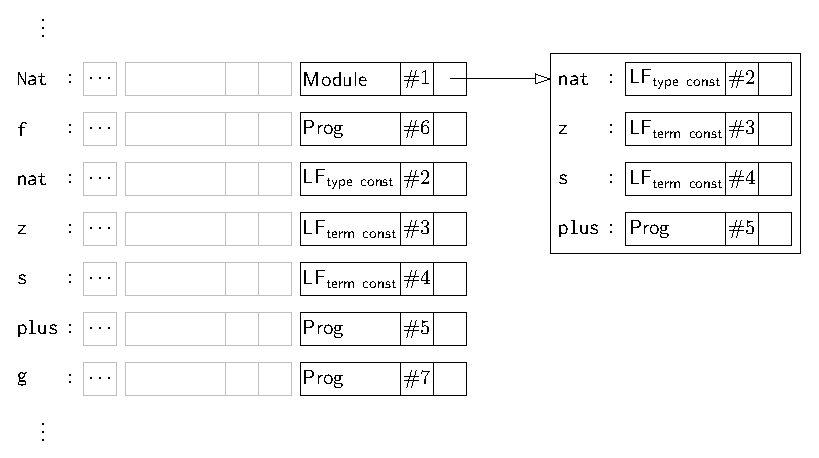
\includegraphics{figures/referencing-environment-implementation.eps}
\caption[Example referencing environment in the implementation]{%
Diagram of the referencing environment at hole \texttt{\verbhole{?h3}} from figure~\ref{figure:referencing-environment-example} as it is implemented in \Beluga~\texttt{v1.1} using dictionaries and stacks.
The identifiers on the left are part of the toplevel module frame, and are each associated with a stack of bindings, with the most recent binding on the right end of the stack.
The numbers \texttt{\#1}, \texttt{\#2}, ..., \texttt{\#7} denote the symbolic identifiers associated with the constants in the signature reconstruction store.
The aliases introduced by opening module \texttt{Nat} are properly handled, such that constant \texttt{\#3} can be referenced either as \texttt{Nat.z} or \texttt{z} at that point in the signature.
}
\label{figure:referencing-environment-implementation}
\end{figure}

The actual data bound to identifiers in referencing environments depends on the kind of binding and the intended usage of that data structure.
As mentioned earlier, the disambiguation phase keeps track of user-defined notations in its referencing environment by attaching their associated parameters to the constants themselves.
This is also replicated during pretty-printing to recover a textual representation of the \ac{AST} that respects user-defined notations.
Pretty-printing to \HTML further assigns IDs to constants so that references to them can be printed as hyperlinks.

For indexing, data is required in the referencing environment to compute valid de Bruijn indices when variables are looked up.
Counting up to the correct de Bruijn index by traversing the dictionaries and stacks in order of addition like is done in the formalism of section~\ref{section:formalising-unified-indexing} defeats the purpose of using dictionaries to speed up lookups.
Instead, as variables are added to the referencing environment, they are annotated with the size of the corresponding indexing context that immediately precedes their addition.
This is achieved using a separate counter that keeps track of the indexing context size.
These annotations effectively indicate the order of insertion into the indexing context.
The de Bruijn index for a variable can then later be recovered simply by subtracting the current indexing context size with the size that was recorded at the binder for that variable.
In other words, as illustrated in figure~\ref{figure:lf-indexing}, if $\Psi'$ is an indexing context with $x \in \Domain(\Psi')$, and $\Psi$ is the indexing context immediately before that $x$ was added, then $|\Psi'| > |\Psi|$ and the de Bruijn index of $x$ with respect to $\Psi'$ is
\begin{equation*}
\mathsf{index}_{\Psi'}(x) = |\Psi'| - |\Psi|.
\end{equation*}
In effect, this is the same computation as subtracting the de Bruijn level of $x$ from the current abstraction depth~\cite{DEBRUIJN1972381, debruijnlevels1995}.
This approach is scalable to arbitrarily many indexing contexts, provided that the context to use for a variable is known at its binding site.
This is the case in \Beluga, where variables in $\Psi$, $\Delta$ and $\Gamma$ are indexed separately and have distinct binders.
Additionally, this approach simplifies shifting contexts in cases like $\mathsf{const} = \lambda x.\lambda\_.\ x$ wherein the identifier introduced by a binder is omitted since it is unused in the abstraction's body.
Indeed, it suffices to increase the indexing context's size to shift it, so there is no need to add an empty binding in the referencing environment.

\begin{figure}[htb]
\centering
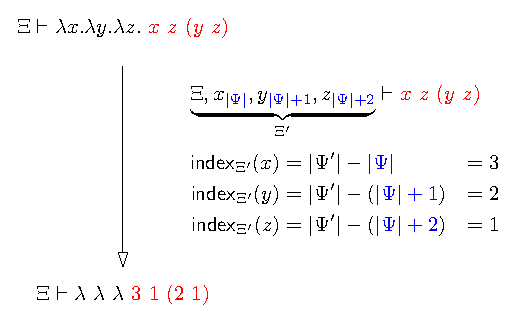
\includegraphics{figures/lf-indexing.eps}
\caption[Example of de Bruijn indices computation with respect to a lookup table]{%
Computation of de Bruijn indices for the $\mathbf{S}$-combinator using indexing context sizes stored in the lookup table.
The bindings of the \LF context $\Psi$ are included in the referencing environment $\Xi$.
The expression $x\ z\ (y\ z)$ is indexed with respect to $\Psi'$ having $|\Psi| + 3$ entries since $x$, $y$ and $z$ are introduced by \LF~abstractions.
Variables in $\Psi'$ are annotated with the size of the \LF indexing context before each of them was added.
}
\label{figure:lf-indexing}
\end{figure}

\section{Discussion}

As part of the reimplementation of the indexing phase, the referencing environment was first designed using immutable data structures.
Specifically, \acp{HAMT} were leveraged for the dictionaries mapping identifiers to stacks of bindings.
The indexing functions were then implemented using the state monad so that derived states could be passed on to later operations.
The motivation for using an immutable data structure was to get copies of the referencing environment for free during indexing.
These copies could then be attached to proof declarations to allow rollbacks like in \Isabelle/\Isar with its context graphs.
In turn, checking out an incomplete theorem in \Harpoon would simply result in the referencing environment's copy being used for elaborating commands.
Unfortunately, the increased number of memory allocations and the lack of contiguity in the memory layout for the referencing environment incurred a decrease in runtime performance by a factor of 10 for \Beluga's test suite.
This meant that running the indexing phase on a signature would take more time than type-checking it.
Thankfully, the indexing phase's implementation was loosely coupled with the representation of the referencing environment, and the state monad was used throughout.
As such, it was easy to shift back to a mutable data structure and recover runtime performance comparable to that of the legacy implementation of \Beluga.
As a consequence, checking out incomplete proofs in \Harpoon involves reconstructing the referencing environment using the internal \ac{AST}'s representation of the signature.

% TODO: Discuss scope graphs as an alternative to the formalism and implementation, argue this end up being the same as association lists because of telescopes

From a programming language implementation standpoint, the revised indexing phase simplified the system's flow of information by decoupling it from the signature reconstruction store.
This opens up multiple opportunities, including proper unit-testing of the referencing environment structure and indexing functions.
Additionally, given \Beluga's design for signature-level declaration of constants, the indexing phase can be parallelized.
This is because the body of a signature-level declaration is guaranteed not to export non-constant identifiers.
This means that the referencing environment right before a signature-level can be constructed while disregarding most of the \ac{AST}.
As such, the declarations in a signature can first be traversed to preallocate symbolic identifiers for toplevel constants and store them in a queue.
Concurrent threads can then be assigned non-overlapping ranges of declarations to process, and the initial referencing environment for each can be constructed using only that queue.
Should this isolation for signature-level declarations be extended to the later phases of processing, concurrently type-checking programs could improve \Beluga's performance.
